\documentclass[a4paper, 12pt]{article}

\usepackage{xcolor}
\usepackage{mdframed}
\definecolor{shadecolor}{rgb}{0.1,0.1,0.1}
\usepackage[utf8]{inputenc}
\usepackage[T1]{fontenc}
\usepackage{textcomp}
\usepackage{amssymb}
\usepackage{amsmath, amssymb}
\usepackage{newtxtext} \usepackage{newtxmath}
\newtheorem{problem}{Problem}
\newtheorem{example}{Example}
\newtheorem{lemma}{Lemma}
\newtheorem{theorem}{Theorem}
\newtheorem{problem}{Problem}
\newtheorem{example}{Example} \newtheorem{definition}{Definition}
\newtheorem{lemma}{Lemma}
\newtheorem{theorem}{Theorem}
\DeclareMathAlphabet{\mathcal}{OMS}{cmsy}{m}{n}
\usepackage[pdftex]{graphicx}
\DeclareGraphicsExtensions{.pdf,.jpeg,.png,.jpg}
\newmdenv[backgroundcolor=orange!25,
            leftline=false,
            rightline=false,
            bottomline=true,
            linewidth=2pt,
            linecolor=black]{myframe}
\newmdenv[backgroundcolor=blue!35,
            leftline=false,
            rightline=false,
            bottomline=true,
            linewidth=2pt,
            linecolor=black]{helpframe}


\begin{document}


\begin{titlepage}
   \begin{center}
       \vspace*{1cm}

       \Huge
       \textbf{Modelos y simulación - Prácticos}

       \vspace{0.5cm}
        FAMAF - UNC
            
       \vspace{1.5cm}
       \large
       \textbf{Severino Di Giovanni}
       \normalsize


       \vspace{5.0cm}
       \begin{figure}[h!]
       \centering
        
\includegraphics[width=0.5\textwidth]{../Images/UPA.jpg}
       \end{figure}

       \vfill
            
            
     
   \end{center}
\end{titlepage}


\shipout\null

 \begin{figure}[h!]
 \centering
  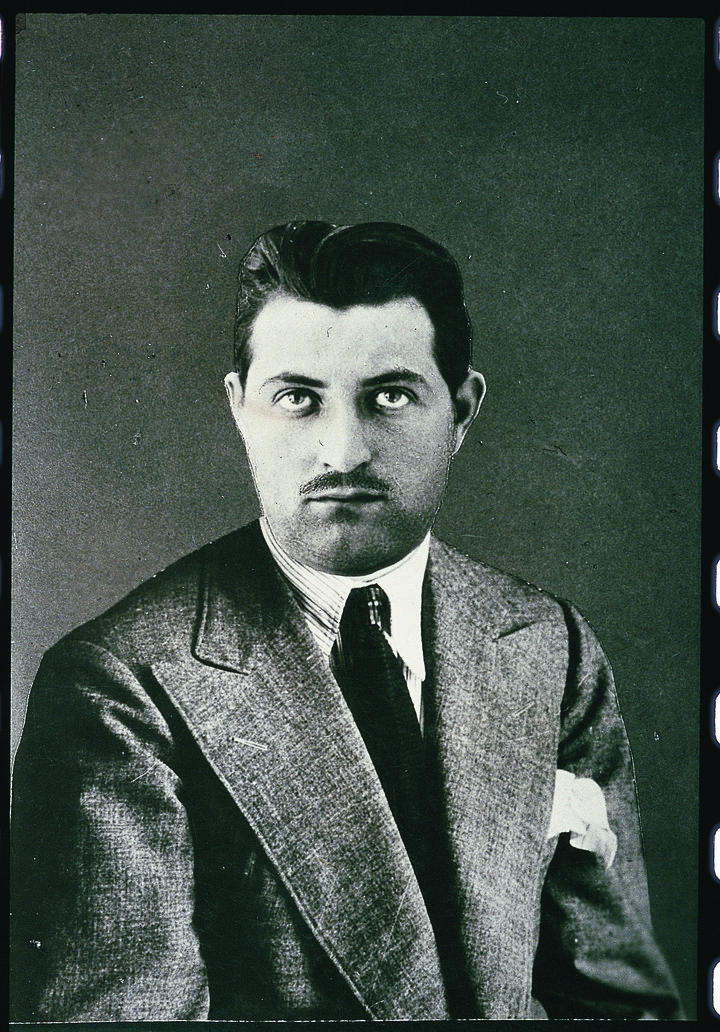
\includegraphics[width=0.5\textwidth]{../Images/SeverinoDiGiovanni.jpg}
 \caption{Severino Di Giovanni, el autor de este apunte. Un anarquista
   libertario, murió luchando por la libertad. Como él, otros miles han muerto
   para que nosotros gocemos de los derechos que tenemos. No te dejes engañar
   por los tristes pregoneros del egoísmo. Amá a tu prójimo y no olvides que si
   sus derechos se vulneran, los tuyos también. Ayudá a tu compañero de estudio,
 defendé tu universidad. }
 \end{figure}

\pagebreak
\tableofcontents
\newpage

\section{Práctico 4: Lenguaje imperativo simple}

\begin{myframe}
(\textbf{1}) Demostrar o refutar.

$(c)$ $(\textbf{if } b \textbf{ then } c_0 \textbf{ else } c_1);c_2 \equiv
\textbf{if } b \textbf{ then } c_0;c_2 \textbf{ else } c_1;c_2$

$(d)$ $c2; (\textbf{if } b \textbf{ then } c0 \textbf{ else } c1) \equiv \textbf{if } b
\textbf{ then } c2; c0 \textbf{ else } c_2; c_1$
\end{myframe}


$(c)$ Sea $p = \textbf{if } b \textbf{ then } c_0 \textbf{ else } c_1$ y

\begin{equation*}
  f = \llbracket \textbf{if } b \textbf{ then } c_0;c_2 \textbf{ else } c_1;c_2
  \rrbracket = \sigma \mapsto \begin{cases}
    \llbracket c_0;c_2 \rrbracket \sigma & \llbracket b \rrbracket \sigma \\ 
    \llbracket c_1;c_2 \rrbracket \sigma & c.c.
  \end{cases}
\end{equation*}

Deseamos probar que $\llbracket p;c_2 \rrbracket = f$. Por def. 

\begin{align*}
  \llbracket p;c_2 \rrbracket \sigma
  &= \llbracket c_2 \rrbracket_{\Bot}\left( \llbracket p \rrbracket \sigma \right) \\ 
  &= \begin{cases}
    \llbracket c_2 \rrbracket_{\Bot} \left(\llbracket c_0 \rrbracket
      \sigma\right) &
    \llbracket b \rrbracket ~ \sigma \\ 
    \llbracket c_2 \rrbracket_{\Bot} \left(\llbracket c_1 \rrbracket
      \sigma\right) & c.c.
  \end{cases} \\ 
  &= \begin{cases}
    \llbracket c_2;c_0 \rrbracket \sigma & \llbracket b \rrbracket \sigma \\ 
    \llbracket c_2;c_1 \rrbracket \sigma & c.c.
  \end{cases}
\end{align*}

$\therefore \llbracket p;c_2 \rrbracket = f$.

~

\begin{align*}
  (d) ~ \llbracket c_2;\textbf{if } b \textbf{ then } c_0 \textbf{ else } c_1 \rrbracket 
  &= \llbracket \textbf{if } b \textbf{ then } c_0 \textbf{ else } c_1
  \rrbracket_{\Bot} \left( \llbracket c_2 \rrbracket \sigma \right)  \\ 
  &= \begin{cases}
    \llbracket \textbf{if } b \textbf{ then } c_0 \textbf{ else } c_1 \rrbracket
    \left( \llbracket c_2 \rrbracket \sigma\right) & \llbracket c_2 \rrbracket
    \sigma \neq \bot  \\ 
    \bot & c.c.
  \end{cases} \\ 
  &= \begin{cases}
    \llbracket c_0 \rrbracket \left( \llbracket c_2 \rrbracket \sigma \right) &
    \llbracket c_2 \rrbracket \sigma \neq \bot \land \llbracket b \rrbracket
    \sigma \\
    \llbracket c_1 \rrbracket \left( \llbracket c_2 \rrbracket \sigma \right) &
    \llbracket c_2 \rrbracket \sigma \neq \bot \land \neg \llbracket b
    \rrbracket \sigma \\ 
    \bot  & \llbracket c_2 \rrbracket\sigma = \bot 
  \end{cases} \\ 
  &= \begin{cases}
    \llbracket c_2;c_0 \rrbracket \sigma &
    \llbracket c_2 \rrbracket \sigma \neq \bot \land \llbracket b \rrbracket
    \sigma \\
    \llbracket c_2;c_1 \rrbracket \sigma &
    \llbracket c_2 \rrbracket \sigma \neq \bot \land \neg \llbracket b
    \rrbracket \sigma \\ 
    \bot  & \llbracket c_2 \rrbracket\sigma = \bot 
  \end{cases} \\ 
  &=\begin{cases}
    \llbracket c_2;c_0 \rrbracket \sigma & ~~~\llbracket b \rrbracket \sigma \\ 
    \llbracket c_2;c_1 \rrbracket \sigma & \neg \llbracket b \rrbracket \sigma
  \end{cases} \\ 
  &= \llbracket \textbf{if } b \textbf{ then } c_2;c_0 \textbf{ else } c_2;c_1
  \rrbracket \sigma
\end{align*}

\pagebreak 

\begin{myframe}
\textbf{(5)} $(a)$ Dar la semántica de $\textbf{while } x < 2 \textbf{ do }  \textbf{if } x <
0\textbf{ then } x := 0 \textbf{ else } x := x + 1$. 
\end{myframe}

\begin{helpframe}
  
\textbf{Razonamiento previo.} Si $\sigma ~ x < 2$, el \textbf{while} incrementa $x$ hasta alcanzar el valor $2$, por lo que su semántica converge a:

\[
\sigma \mapsto 
\begin{cases}
\sigma & \sigma ~ x \geq 2 \\
[\sigma \mid x : 2] & \sigma ~ x < 2
\end{cases}
\]

En el peor caso ($\sigma ~ x < 0$), el bucle realiza a lo sumo $3$ iteraciones: una para corregir $x < 0$, y dos más para alcanzar $2$.

De esto se sigue que: (1) el bucle siempre termina en a lo sumo $3$ pasos, y (2)
sólo $F^1 ~ \bot$ a $F^4 ~ \bot$ aportan información; luego, la cadena se vuelve
no interesante.
\end{helpframe}

Por simplicidad, hagamos $p := \textbf{if } x < 0 \textbf{ then } x:=0 \textbf{
else } x := x+1$ y observemos que

\begin{equation}
  \llbracket p \rrbracket \sigma = \begin{cases}
    [\sigma \mid x : 0] & \sigma ~x < 0 \\ 
    [\sigma \mid x : \sigma ~ x + 1] & \sigma~ x \geq 0
  \end{cases}
\end{equation}

Definamos $F : (\Sigma
\mapsto \Sigma_\bot ) \mapsto (\Sigma \mapsto \Sigma_\bot )$ como 

\begin{equation*}
  F ~ f ~ \sigma = \begin{cases}
    \sigma & \sigma ~ x \geq 2 \\ 
    f_{\Bot} ~ \llbracket p \rrbracket ~ \sigma & \sigma ~ x < 2
  \end{cases}
\end{equation*}

Aplicando $(1)$, obtenemos


\begin{equation*}
  F ~ f ~\sigma = \begin{cases}
    \sigma & \sigma ~ x \geq 2 \\ 
    f \left( [\sigma \mid x : \sigma ~ x + 1] \right) & \sigma ~ x \in \left\{
    0, 1 \right\} \\
    f \left( [\sigma \mid x : 0] \right) &\sigma ~ x < 0
  \end{cases}
\end{equation*}

Es trivial observar que

\begin{equation*}
  F ~ \bot ~ \sigma 
  &=\begin{cases}
    \sigma & \sigma ~ x \geq 2 \\
    \bot &\sigma ~ x < 2
  \end{cases}
\end{equation*}

Ahora bien,

\begin{align*}
  F^2 ~ \bot ~ \sigma 
  &=\begin{cases}
    \sigma & \sigma ~ x \geq 2 \\ 
    (F ~ \bot ) \left( [\sigma \mid x : \sigma ~ x + 1] \right) & \sigma ~ x \in \left\{
    0, 1 \right\} \\
      (F ~ \bot ) \left( [\sigma \mid x : 0] \right) &\sigma ~ x < 0
  \end{cases}
\end{align*}

En el caso $\sigma ~ x \in \left\{ 0, 1 \right\} $, tenemos 

\begin{align*}
  (F ~ \bot ) \left( [\sigma \mid x : \sigma ~ x + 1] \right) 
  = \begin{cases}
    F([\sigma \mid x : 2]) & \sigma ~ x = 1 \\ 
    F([\sigma \mid x : 1]) & \sigma ~ x = 0
  \end{cases} = \begin{cases}
    [\sigma \mid x : 2] & \sigma ~ x = 1 \\ 
    \bot  & \sigma ~ x = 0
  \end{cases}
\end{align*}


En el caso $\sigma ~ x < 0$, claramente $F([\sigma \mid x < 0]) = \bot $. Con lo
cual 

\begin{equation*}
  F^2 ~ \bot  ~ \sigma = \begin{cases}
    \sigma & \sigma ~ x \geq 2 \\ 
    [\sigma \mid x : 2] & \sigma ~ x = 1 \\ 
    \bot  & \sigma ~ x < 1
  \end{cases}
\end{equation*}

De manera análoga se demuestra que 

\begin{equation*}
  F^3 ~ \bot  ~ \sigma = \begin{cases}
    \sigma & \sigma ~ x \geq 2 \\ 
    [\sigma \mid x : 2] & \sigma ~ x \in  \left\{ 0,1 \right\}  \\ 
    \bot  & \sigma ~ x < 1
  \end{cases}
\end{equation*}

Entonces

\begin{align*}
  F^4 ~ \bot ~ \sigma 
  &=\begin{cases}
    \sigma & \sigma ~ x \geq 2 \\ 
    (F^3 ~ \bot ) \left( [\sigma \mid x : \sigma ~ x + 1] \right) & \sigma ~ x \in \left\{
    0, 1 \right\} \\
      (F^3 ~ \bot ) \left( [\sigma \mid x : 0] \right) &\sigma ~ x < 0
  \end{cases} \\ 
  &=\begin{cases}
    \sigma & \sigma ~ x \geq 2 \\ 
    [\sigma \mid x : 2] & \sigma ~ x < 2
  \end{cases}
\end{align*}

Es obvio entonces que a partir de $k \geq 4$, $F^{k+1} \bot  = F^k \bot $, con
lo cual $F^1 ~ \bot, F_2 ~ \bot , \ldots$ es una cadena no interesante con
supremo $F^4 ~ \bot $.

\begin{equation*}
  \therefore ~ \bigsqcup_{i \in \mathbb{N}} F^{i} ~ \bot = \lambda \sigma. \begin{cases}
    \sigma & \sigma ~ x \geq 2 \\ 
    [\sigma \mid x : 2] & \sigma ~ x < 2
  \end{cases} = \llbracket \textbf{if } \sigma ~ x \geq 2 \textbf{ then }
  \textbf{skip} \textbf{ else } \sigma ~ x := 2 \rrbracket
\end{equation*}


\pagebreak

\begin{myframe}
  \textbf{(5)} $(b)$ Dar la semántica de 

  $$\textbf{while } x < 2 \textbf{ do } \textbf{if } y = 0 \textbf{ then } x :=
  x+1 \textbf{ else } \textbf{skip }$$
\end{myframe}

Debería ser claro que si $y \neq 0$ el ciclo no termina, pues se ejecuta
$\textbf{skip}$ indefinidamente. 

Sea $p$ el comando \textbf{if} ejecutado dentro del \textbf{while}. Si definimos $F : (\Sigma \mapsto \Sigma_\bot )
\mapsto (\Sigma \mapsto \Sigma_\bot )$ como 

\begin{equation*}
  F ~ f ~ \sigma = \begin{cases}
    \sigma & \sigma ~ x \geq 2 \\ 
    f_{\Bot} \left( ~ \llbracket p \rrbracket \sigma\right) & \sigma ~ x < 2
  \end{cases}
\end{equation*}

entonces, desarrollando la semántica de $p$, tenemos 

\begin{equation*}
  F ~ f ~ \sigma = \begin{cases}
    \sigma & \sigma ~ x \geq 2 \\ 
    f_{\Bot} \left( [\sigma \mid x : \sigma ~ x + 1] \right)  & \sigma ~ x < 2
    \land \sigma ~ y = 0 \\
    f_{\Bot} \sigma  & \sigma ~ x < 2 \land \sigma ~ y \neq 0
  \end{cases}
\end{equation*}

Ahora daremos el menor punto fijo de $F$, que será la semántica del comando.
Claramente, 

\begin{equation*}
  F ~ \bot ~ \sigma = \begin{cases}
    \sigma & \sigma ~ x \geq 2 \\ 
    \bot & \text{c. c.}
  \end{cases}
\end{equation*}

Continuando,

\begin{align*}
  F^2 ~ \bot  ~ \sigma 
  &= \begin{cases}
    \sigma & \sigma ~ x \geq 2 \\ 
    (F ~ \bot )_{\Bot} \left( [\sigma \mid x : \sigma ~ x + 1] \right)  & \sigma ~ x < 2
    \land \sigma ~ y = 0 \\
    (F ~ \bot )_{\Bot} \sigma  & \sigma ~ x < 2 \land \sigma ~ y \neq 0
  \end{cases} \\ 
  &= \begin{cases}
    \sigma & \sigma ~ x \geq 2 \\ 
    [\sigma \mid x : \sigma ~ x + 1] & \sigma ~ x = 1 \land  y = 0 \\ 
    \bot  & \sigma ~ x < 1 \land  y = 0 \\ 
    \bot & \sigma ~ x <2 \land  \sigma ~  y \neq 0
  \end{cases}\\
  &= \begin{cases}
    \sigma & \sigma ~ x \geq 2 \\ 
    [\sigma \mid x : 2] & \sigma ~ x = 1 \land  y = 0 \\ 
    \bot  & \sigma ~ x < 1 \land  y = 0 \\ 
    \bot & \sigma ~ x <2 \land  \sigma ~  y \neq 0
  \end{cases}
\end{align*}

Solo para ser explícitos, veamos que 

\begin{align*}
  F^3 ~ \bot  ~ \sigma 
  &= \begin{cases}
    \sigma & \sigma ~ x \geq 2 \\ 
    (F ~ \bot )^2_{\Bot} \left( [\sigma \mid x : \sigma ~ x + 1] \right)  & \sigma ~ x < 2
    \land \sigma ~ y = 0 \\
    (F ~ \bot )^2_{\Bot} \sigma  & \sigma ~ x < 2 \land \sigma ~ y \neq 0
  \end{cases} \\ 
  &= \begin{cases}
    \sigma & \sigma ~ x \geq 2 \\ 
    [\sigma \mid x : 2] & \sigma ~ x \in \left\{ 0, 1 \right\}  \land  y = 0 \\ 
    \bot  & \sigma ~ x < 0 \land  y = 0 \\ 
    \bot & \sigma ~ x <2 \land  \sigma ~  y \neq 0
  \end{cases}
\end{align*}

Planteamos como hipótesis inductiva que 

\begin{equation*}
  F^k ~ \bot ~ \sigma = \begin{cases}
    \sigma & \sigma ~ x \geq 2 \\ 
    [\sigma \mid x : 2] &3 - k \leq \sigma ~ x \leq 1 \land y = 0 \\ 
    \bot & c.c.
  \end{cases}
\end{equation*}

Entonces 

\begin{align*}
  F^{k+1} ~ \bot ~ \sigma 
  &= \begin{cases}
    \sigma & \sigma ~ x \geq 2 \\ 
    (F ~ \bot )^k_{\Bot} \left( [\sigma \mid x : \sigma ~ x + 1] \right)  & \sigma ~ x < 2
    \land \sigma ~ y = 0 \\
    (F ~ \bot )^k_{\Bot} \sigma  & \sigma ~ x < 2 \land \sigma ~ y \neq 0
  \end{cases} \\ 
  &=\begin{cases}
    \sigma & \sigma ~ x \geq 2 \\ 
    [\sigma \mid x : \sigma ~ x + 1 ] & \sigma ~ x < 2\land \sigma ~ x + 1 \geq
    2 \land  y = 0 \\
    [\sigma \mid x : 2] & \sigma ~ x < 2 \land  3 - k \leq \sigma ~ x + 1 \leq 1 \land  y = 0 \\ 
    \bot & c.c.
  \end{cases} \\ 
  &=\begin{cases}
    \sigma & \sigma ~ x \geq 2 \\ 
    [\sigma \mid x : 2] & \sigma ~ x < 2 \land  \sigma ~ x \geq 1 \land  y  =0
    \\ 
    [\sigma \mid x : 2] & \sigma ~ x < 2 \land 3 - (k+1) \leq \sigma ~ x \leq 0
    \land  y  = 0 \\ 
    \bot  &c.c.
  \end{cases}\\
  &=\begin{cases}
    \sigma & \sigma ~ x \geq 2 \\ 
    [\sigma \mid x : 2] & \sigma ~ x = 1\land   y  =0
    \\ 
    [\sigma \mid x : 2] & 3 - (k+1) \leq \sigma ~ x \leq 0
    \land  y  = 0 \\ 
    \bot  &c.c.
  \end{cases}\\
  &=\begin{cases}
    \sigma & \sigma ~ x \geq 2 \\ 
    [\sigma \mid x : 2] & 3 - (k+1) \leq \sigma ~ x \leq 1
    \land  y  = 0 \\ 
    \bot  &c.c.
  \end{cases}
\end{align*}

\textit{quod erat demonstrandum}. Se sigue entonces que 

\begin{equation*}
  \bigsqcup_{i \in \mathbb{N}} F^{i} ~ \bot = \lambda \sigma . \begin{cases}
    \sigma & \sigma ~ x \geq 2 \\ 
    [\sigma \mid x : 2] &\sigma ~ x \leq 1 \land  y = 0 \\ 
    \bot & \sigma ~ y \neq 0
  \end{cases}
\end{equation*}

\footnotesize
\begin{helpframe}
  \textbf{Aclaración.} Para no escribir tanto, agrupamos $\bot $ en un solo caso
  durante el desarrollo de $F^1 ~ \bot , F^2 ~ \bot $, etc. Pero debería ser
  claro que en uno de los casos damos $\bot $ porque la cantidad de iteraciones
  es limitada, mientras que en otro caso damos $\bot $ porque $\sigma ~ y \neq 0$. En el
  primer caso, a medida que se aumentan las iteraciones, se añade más y más
  información y, en el límite, la indefinición desaparece. En el segundo caso,
  la indefinición no desaparece: siempre que $\sigma ~ y \neq 0$, se da $\bot $.
\end{helpframe}

\pagebreak 

\begin{myframe}
  \textbf{(6)} Asuma que $\llbracket \textbf{while } b \textbf{ do } c\rrbracket\sigma \neq
  \bot $. Demuestre $(a)$ que existe $n \geq 0$ tal que $F^n ~ \bot ~ \sigma
  \neq \bot $. Demuestre $(b)$ que si $\sigma' = \llbracket \textbf{while } b
  \textbf{ do } c\rrbracket\sigma$, entonces $\neg\llbracket b
  \rrbracket\sigma'$.
\end{myframe}

$(a)$ Sabemos que 

\begin{equation*}
  \llbracket \textbf{while } b \textbf{ do } c\rrbracket = \bigsqcup_{i \in
  \mathbb{N}} F^i ~ \bot 
\end{equation*}

para 

\begin{equation*}
  F ~ f ~ \sigma = \begin{cases}
    \sigma & \neg\llbracket b \rrbracket \sigma \\ 
    f_{\Bot}\llbracket c \rrbracket\sigma & c.c.
  \end{cases}
\end{equation*}

Asuma que no existe $n \geq 0$ tal que $F^n ~ \bot  ~ \sigma \neq \bot $. Se
sigue que la cadena $\left\{ F^i ~ \bot  \right\}_{i \in \mathbb{N}} $ es
simplemente la cadena $\bot  \sqsubseteq \bot \sqsubseteq \bot  \sqsubseteq
\ldots$. El supremo de esta cadena es $\bot $. Por lo tanto, 

\begin{equation*}
  \llbracket \textbf{while } b \textbf{ do } c\rrbracket = \bigsqcup_{i \in
  \mathbb{N}} F^i ~ \bot = \bot 
\end{equation*}

lo cual contradice la hipótesis. La contradicción viene de asumir que no existe
$n \geq 0$ tal que $F^n ~ \bot  ~ \sigma \neq \bot $. 

$\therefore $ Existe $n \geq 0$ tal que $F^n ~ \bot ~ \sigma \neq \bot. \qquad
\blacksquare $

$(b)$  Dado que la semántica de $\textbf{while } b \textbf{ do } c$ es un
punto fijo de $F$, si usamos $\varphi := \llbracket \textbf{while } b \textbf{
do } c \rrbracket$, entonces

\begin{equation*}
  \varphi ~ \sigma = F ~ \varphi ~ \sigma
\end{equation*}

Si $\sigma$ es tal que $\neg \llbracket b \rrbracket\sigma$, entonces se sigue
inmediatamente de la definición de $F$ que en el estado $\varphi \sigma$ no se
cumple $b$. Veamos el caso en que se cumple $\llbracket b \rrbracket\sigma$.
Por la definición de $F$, 


\begin{equation}
  \varphi ~ \sigma = \varphi_{\Bot}\left( \varphi_{\Bot} \ldots \left(
  \varphi_{\Bot}\llbracket c \rrbracket \sigma \right)  \right) =
  \varphi_{\Bot}^k \llbracket c \rrbracket\sigma
\end{equation}

donde la hipótesis de que el ciclo nunca es $\bot$ nos permite garantizar que
existe tal $k \in \mathbb{N}$. Ahora bien, por la definición de $F$, $k$ es
definido estrictamente por el hecho de que

\begin{equation*}
  \neg \llbracket b \rrbracket( \varphi^k_{\Bot}\llbracket c \rrbracket\sigma )
\end{equation*}

Por la ecuación $(2)$, resulta entonces 

\begin{equation*}
  \neg\llbracket b \rrbracket\left( \varphi \sigma \right) \quad \blacksquare
\end{equation*}

\pagebreak 

\begin{myframe}
  \textbf{(7)} Demostrar o refutar:

  $(a)$ $\textbf{while } \textbf{false do } c \equiv \textbf{skip}$

  $(b)$ $\textbf{while } b \textbf{ do } c \equiv \textbf{while } b \textbf{ do
  } (c;c)$ 

  $(c)$  $(\textbf{while } b \textbf{ do } c); \textbf{if } b \textbf{ then }
  c_0 \textbf{ else } c_1 \equiv (\textbf{while } b \textbf{ do } c); c_1$
\end{myframe}

$(a)$ Es trivial.

~ 

$(b)$ Falso. Basta dar un contraejemplo. Sea $\sigma$ un estado con $\sigma ~ x
= 0$ y considere 

\begin{equation*}
  w_1 := \textbf{while } x \leq 0 \textbf{ do } x := x + 1, \qquad w_2 :=
  \textbf{while } x \leq 0 \textbf{ do } ( x := x + 1 );(x := x + 1)
\end{equation*}

Claramente, $\llbracket w_1 \rrbracket\sigma ~ x = 1$ y $\llbracket w_2
\rrbracket\sigma ~ x = 2$. Sin embargo, dados comandos $c_1,c_2$,

\begin{equation*}
  c_1 \equiv c_2 \iff \forall \sigma \in \Sigma: \llbracket c_1 \rrbracket\sigma = \llbracket c_2
  \rrbracket\sigma
\end{equation*}

$\therefore ~ w_1 \not\equiv w_2$. 

$(c)$ Es verdadero. En el ejercicio anterior, demostramos que si un ciclo termina, entonces la
guarda no puede cumplirse en el estado resultante del ciclo. Es decir que si 

\begin{equation*}
  \llbracket \textbf{while } b \textbf{ do } c \rrbracket\sigma = \sigma' \neq
  \bot 
\end{equation*}

entonces $\llbracket b \rrbracket \sigma' \equiv
\textbf{False}$. Por lo tanto, asumiendo que $\llbracket \textbf{while } b
\textbf{ do } c \rrbracket\sigma$ termina y no es $\bot $,

\begin{align*}
  &\llbracket ( \textbf{while } b \textbf{ do } c );\textbf{if } b \textbf{ then
  } c_0 \textbf{ else } c_1 \rrbracket\sigma \\ 
  =~&\llbracket \textbf{if } b \textbf{ then } c_0 \textbf{ else } c_1
  \rrbracket\left( \llbracket \textbf{while } b \textbf{ do } c \rrbracket\sigma
  \right) \\ 
  =~&\llbracket c_1 \rrbracket \left( \llbracket \textbf{while } b \textbf{ do }
   c \rrbracket\sigma \right)  \\ 
  = ~ &\llbracket ( \textbf{while } b \textbf{ do } c );c_1 \rrbracket\sigma \qquad
  \blacksquare
\end{align*}

Ahora bien, si el ciclo no termina (es decir, si devuelve $\bot$), es trivial
demostrar que la equivalencia también se cumple.

\pagebreak 

\begin{myframe}
  \textbf{(8)} Considerar las siguientes definiciones como syntactic sugar del
  comando $$\textbf{for } v := e_0 \textbf{ to } e_1 \textbf{ do } c$$

  $(a)$ $v := e_0; \textbf{while } v \leq e_1 \textbf{ do } c; v := v + 1$

  $(b)$ $\textbf{newvar } v := e_0 \textbf{ in } \textbf{while } v \leq e_1
  \textbf{ do } c; v := v+1$

  $(c)$ $\textbf{newvar } w := e_1 \textbf{ in newvar } v := e_0 \textbf{ in
  while } v \leq w \textbf{ do } c; v := v+1$

  ¿Es alguna satisfactoria? Justificar.
\end{myframe}

Recordemos que, al menos de acuerdo con Reynolds,

\begin{align*}
  &\textbf{for } v := e_0 \textbf{ to } e_1 \textbf{ do } c \\ 
  := ~ &\textbf{newvar } w := e_1 \textbf{ in newvar } v:= e_0 \textbf{ in while
  } v \leq w \textbf{ do } (c; v := v+1)
\end{align*}

que es la expresión $(c)$. Para no ser tramposos, igual justificaremos por qué
dicha definición es satisfactoria, llegado el momento.

~ 

$(a)$ La definición es satisfactoria en el sentido de que, si se la llama en un
estado $\sigma$, ejecutará el comando
$c$ en los sucesivos estados 

\begin{align*}
  &[\sigma \mid v : \llbracket e_0 \rrbracket\sigma]\\ 
  &[\sigma \mid v : \llbracket e_0 \rrbracket\sigma + 1]\\
  &\vdots\\
  &[\sigma \mid v : \llbracket e_1 \rrbracket\sigma]
\end{align*}

Sin embargo, debemos notar que no se restaura el valor de $v$, i.e. $v$ no es
local al ciclo.

~

$(b)$ Esta definición es funcional y restaura el valor de $v$. Sin embargo, es
ineficiente, porque en cada llamada del while debe volver a computarse el valor
de $e_1$ bajo el estado dado. Es concebible que $e_1$ sea una expresión
compleja, e.g. una productoria de $k > 10.000$ variables, o cualquier locura que
se nos ocurra. Por lo tanto, lo ideal sería computar la cota superior $e_1$ una
sola vez y alocar dicho valor en otra variable.

~

$(c)$ La definición $(c)$ resuelve el problema de la $(b)$, porque aloca en la
variable local $w$ el valor de la cota superior, que por lo tanto se computa una
única vez. Una vez dicho valor es asignado a $w$, procede igual que en la def.
$(b)$: asigna a una variable local $v$ el valor de $e_0$ e itera adecuadamente.

\pagebreak 

\begin{myframe}
  \textbf{(10)} Enunciar el teorema de coincidencia  y demostra el caso $\textbf{while}$.
\end{myframe}

\begin{helpframe}
  \textbf{Teorema de coincidencia.} 

  $(a)$ Sean $\sigma, \sigma'$ estados tales
  que $\sigma ~ w = \sigma' ~ w$ para toda $w \in FV(c)$. Entonces o bien 
  $\llbracket c \rrbracket\sigma = \llbracket c \rrbracket\sigma' = \bot $ o
  bien 
  $\llbracket c \rrbracket\sigma ~ w = \llbracket c \rrbracket\sigma' ~ w$ para
  toda $w \in FV(c)$.

  ~

  $(b)$ Si $\llbracket c \rrbracket\sigma \neq \bot $, entonces $\llbracket c
  \rrbracket\sigma ~ w = \sigma ~ w$ para toda $w \in FA(c)$.
\end{helpframe}


$(a)$ Sean $\sigma_1, \sigma_2$ tales que $\sigma_1 ~ w = \sigma_2 ~ w$ para
todo $w \in FV(c)$, donde 

\begin{equation*} c := \textbf{while } b \textbf{ do } d \end{equation*}

Por def. de $FV$, tenemos que $\sigma_1 ~ w = \sigma_2 ~ w$ para toda $w \in
FV(b) \cup FV(d)$. Asumamos como hipótesis inductiva que el teorema vale para $b$ y $d$, y definamos


\begin{align*}
  \gamma_1 := \llbracket d \rrbracket\sigma_1, \qquad \gamma_{i+1} := \llbracket d
  \rrbracket\gamma_i\\
  \beta_1 := \llbracket d \rrbracket\sigma_2, \qquad \beta_{i+1} := \llbracket d
  \rrbracket\beta_i
\end{align*}

Es decir, $\left\{ \gamma_i \right\} $ y $\left\{ \beta_i \right\} $ son los
estados correspondientes a las sucesivas iteraciones del \textbf{while}.
Observemos que por HI resulta que $\gamma_1 = \llbracket d \rrbracket\sigma_1,
\beta_1 = \llbracket d \rrbracket\sigma_2$ coinciden en las variables libres de
$d$. Es fácil ver por inducción que entonces $\gamma_i, \beta_i$ coinciden en
las variables libres de $d$ para toda $i$.

~ 

Observemos que $b$ no tiene variables ligadas y por lo tanto, o bien es
constante, o bien posee sólo variables libres. Si $b$ es constante el problema
es trivial porque o bien el while se ejecuta indefinidamente desde cualquier
estado, o no se ejecuta desde ningún estado. Así que veamos el caso en que $b$
tiene al menos una variable libre.

~ 

Observemos que si $b$ y $d$ no tienen variables libres en común, entonces las
sucesivas ejecuciones de $d$ no afectarán el valor de $b$ y, por lo tanto, o
bien el \textbf{while} se ejecuta sin terminar desde ambos estados, o no se
ejecuta desde ninguno de los estados. Así que en este caso el problema es
trivial. Por lo tanto, veamos el caso $FV(b) \cap FV(d) \neq \emptyset$.


~

Demostremos que $(\star) ~  \llbracket b \rrbracket\gamma_i = \llbracket b
\rrbracket\beta_i$. Claramente, una ejecución de $d$ sólo afecta la semántica de
$b$ a través de modificaciones de las variables en $FV(b) \cap FV(d) \subseteq
FV(d)$. Pero ya establecimos que $\gamma_i ~ w = \beta_i ~ w$ para toda
$w \in FV(d)$, y entonces esto es verdadero para el caso particular $w \in FV(b)
\cap FV(d)$. Por lo tanto, $\gamma_i, \beta_i$ coinciden en los valores de las
variables libres de $b$ que también son variables libres de $d$. Respecto a las
variables libres de $b$ que no son variables libres de $d$, las mismas no son
modificadas por las sucesivas ejecuciones de $d$. Por lo tanto tienen el mismo
valor que en $\sigma_1$ y $\sigma_2$, respectivamente. Pero $\sigma_1, \sigma_2$
coinciden en las variables libres de $b$. Por lo tanto, coinciden también en
estas variables.

~

Asuma que $\llbracket c \rrbracket\sigma_1 =\bot $. Entonces, para toda $i$ se
cumple que $\llbracket b \rrbracket\gamma_i \equiv \textbf{True}$ (de otro modo
el \textbf{while} terminaría). Por $(\star)$ se sigue que $\llbracket b
\rrbracket\beta_i \equiv \textbf{True}$. Como esto vale para toda $i$, las
sucesivas iteraciones de $\left\{ \beta_i \right\} $ nunca hacen la guarda
falsa. Por lo tanto, el \textbf{while} nunca termina partiendo desde $\sigma_2$.
$\therefore \llbracket c \rrbracket\sigma_2 = \bot $

~ 

Asuma que $\llbracket c \rrbracket\sigma_1 \neq \bot$. Un razonamiento idéntico
al anterior nos da que $\llbracket c \rrbracket\sigma_2 \neq \bot $, y no sólo
eso sino que se da la misma cantidad $k$ de iteraciones en ambos casos. Es decir
que los estados finales de ambos casos son $\gamma_k, \beta_k$, respectivamente.
Ya observamos antes que $\gamma_k, \beta_k$ coinciden en las variables libres de
$d$ y de $b$, lo cual concluye la prueba.























\end{document}



